% !TEX encoding = UTF-8
% !TEX TS-program = pdflatex
% !TEX root = ../tesi.tex

\subsection{UC6 - Visualizzazione jobs}
\begin{itemize}
  \item \textbf{Identificativo}: UC6
  \item \textbf{Nome}: visualizzazione jobs
  \item \textbf{Descrizione grafica}:
\end{itemize}

\begin{figure}[h]
  \centering
  %  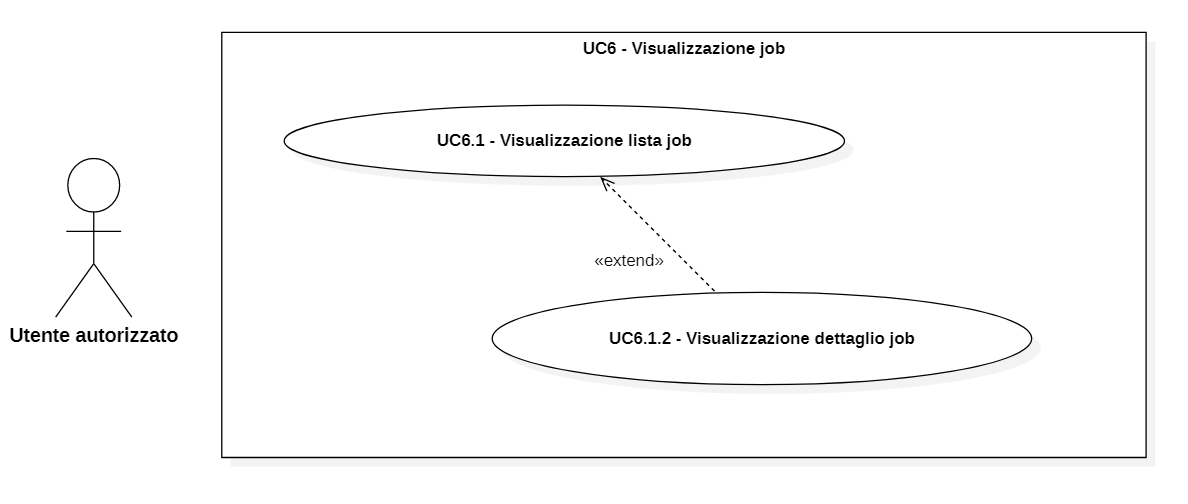
\includegraphics[scale=0.50]{images/UC6.png}
  \caption{Descrizione grafica caso d'uso UC6}
\end{figure}

\begin{itemize}
  \item \textbf{Attori}
        \begin{itemize}
          \item \textit{Primari}: utente autorizzato
        \end{itemize}
  \item \textbf{Precondizione}: l'utente si trova all'interno dell'applicazione e vuole visualizzare la lista dei jobs.
  \item \textbf{Postcondizione}: l'utente visualizza la lista dei jobs.
  \item \textbf{Scenario principale}: l'utente visualizza la lista dei jobs.
  \item \textbf{Scenario secondario}: l'utente può visualizzare il dettaglio di un singolo job premendo sull'apposito link. (\textbf{UC6.1})
\end{itemize}

\subsubsection{UC6.1 - Visualizzazione dettaglio job}
\begin{itemize}
  \item \textbf{Identificativo}: UC6.1
  \item \textbf{Nome}: visualizzazione dettaglio job
  \item \textbf{Descrizione grafica}: (approfondita in UC6)
  \item \textbf{Attori}
        \begin{itemize}
          \item \textit{Primari}: utente autorizzato
        \end{itemize}
  \item \textbf{Precondizione}: l'utente ha premuto sull'apposito link.
  \item \textbf{Postcondizione}: il dettaglio del job viene visualizzato.
  \item \textbf{Scenario principale}: l'utente visualizza tutti i dettagli del singolo job.
\end{itemize}